\documentclass{article}

\usepackage{amsmath}   %% for \cfrac
\usepackage{xcolor}    %% for colored text
\usepackage{pagecolor} %% for dark background
\usepackage{graphicx}  %% for images
\usepackage{geometry}
\usepackage{hyperref}
\usepackage{wrapfig}

\geometry{
a4paper,
total={170mm,257mm},
left=20mm,
right=20mm,
top=20mm
}

\graphicspath{ {../../docs/},{../../../../docs/} }

\pagecolor{black}
\definecolor{magenta}{RGB}{255,0,255}
\definecolor{cyan}{RGB}{0,255,255}
\definecolor{white}{RGB}{255,255,255}
\definecolor{blue}{RGB}{0,0,255}
\definecolor{green}{RGB}{0,255,0}

\begin{document}

\font\titlefont=cmr12 at 30pt

\color{magenta}
\Huge{\title{\vspace{-3cm}\color{magenta}\titlefont Astrodynamics with Python}}
\color{white}
\author{Alfonso Gonzalez}
\date{}
\maketitle

\begin{center}
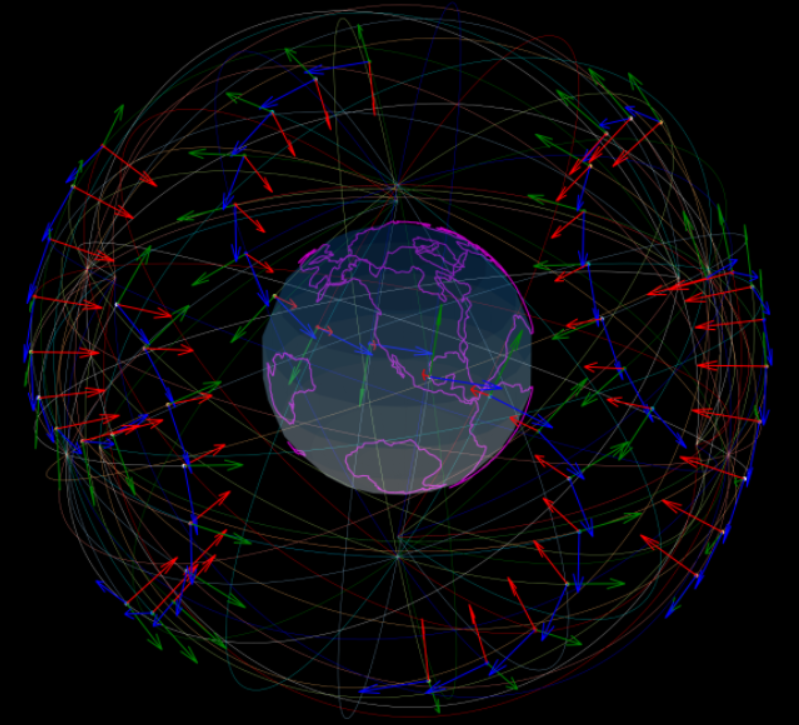
\includegraphics[width=300pt]{prof-pic-hq-centered.png}
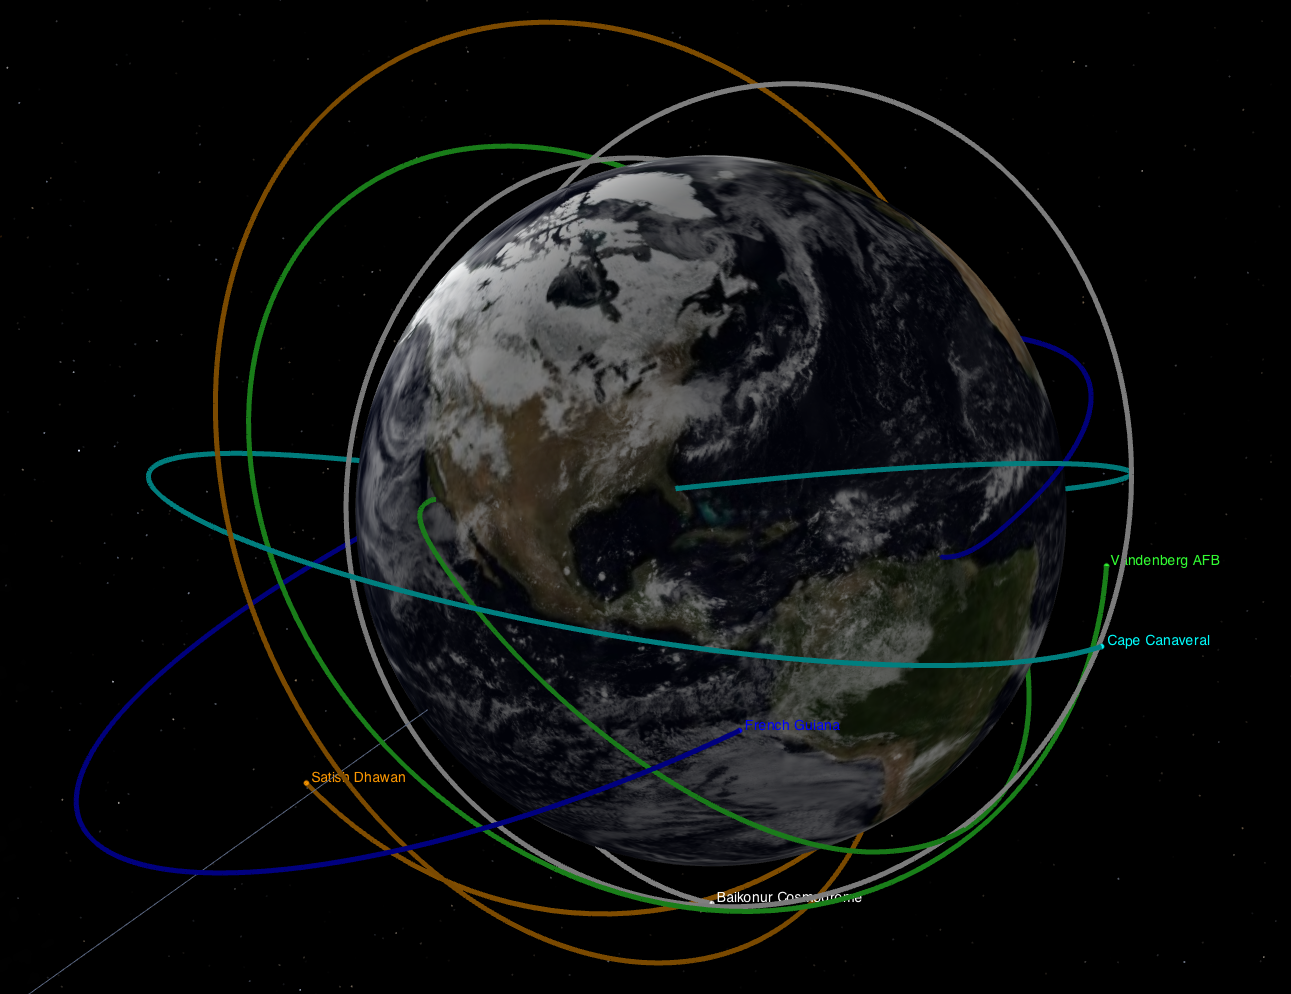
\includegraphics[width=400pt]{cosmo-3d-launches.png}
\end{center}

\newpage

\begin{center}\huge{
\color{magenta}
\hspace{-10pt}
\vfill
To: Mom (Veronica), Dad (Carl), Brother (Alberto) and all past, present, and future humans of Earth, Earth's Moon, Mars, and Beyond. Original writing began in year 2021.
\hspace{15pt}
\vfill
}
\end{center}

\newpage

\textwidth=700pt

\normalsize

\tableofcontents

\newpage

\section{Preface}

The \color{magenta}Astrodynamics with Python \color{white} book, YouTube videos, and GitHub repository are all products
of the simple belief that all information should be free to anyone with access to the internet.
They are collectively my attempt at providing useful information to the world.


Also because of that belief, if you'd like to help me by translating this project to your native language, don't hesitate
to contact me at: \color{magenta}spaceengineeringpodcast@gmail.com \color{white}


This book is unlike other books, given that (for now) it is solely electronic, is being released as its being written (chapter by chapter),
and will be a very iterative process (hence why it is being version controlled via Git). This is for multiple reasons:
\begin{itemize}
	\item Free to anyone with access to the internet
	\item Easy to publish (git push, merge to main)
	\item This is a collaboration with other engineers who contribute by translating
	\item This is a collaboration with readers (you)
	\begin{itemize}
		\item If you see a mistake or are confused by an explanation, reach out
		via email or open up Git Issue, so that when the book is updated, your
		Git Issue will be attached to the fix/improvement git commit, thus you will have
		directly contributed to this project!
		\item This applies to the book as well as the software in this repository.
	\end{itemize}
\end{itemize}

Now lets get to the technical work.

\section{Chapters and Material}
The following are general guidelines of how this book will be written:
\begin{itemize}
	\item Visuals and software will be at the center of every explanation / derivation
	\begin{itemize}
		\item In general, I don't consider myself to truly understand a problem until I can solve it on paper \textbf{AND} implement it in software.
	\end{itemize}

\end{itemize}

\noindent
The current plan is to separate the book by the following topics:
\begin{itemize}
	\item Orbital mechanics
	\item Spacecraft attitude control
	\item Rocket trajectories
	\item Numerical methods
	\item Trajectory optimization
	\item Prerequisites
\end{itemize}
 
The book, videos, and software will all be complementing each other, and will be
continuously updated as needed / requested from the readers.

\newpage

\begin{wrapfigure}{R}{0.3\textwidth}
\centering
\includegraphics[width=0.25\textwidth]{two-body-with-coastlines.png}
\includegraphics[width=0.25\textwidth]{groundtracks.png}
\includegraphics[width=0.25\textwidth]{earth2mars.png}
\includegraphics[width=0.25\textwidth]{EVME.png}
\end{wrapfigure}

\subsection{Orbital Mechanics}
This section of the book will be organized in the same order as the
Fundamentals of Orbital Mechanics video series \color{cyan}
\href{https://www.youtube.com/playlist?list=PLOIRBaljOV8hBJS4m6brpmUrncqkyXBjB}{(link to YouTube playlist)}\color{white}

\noindent
The following are the planned topics:

\begin{itemize}
	\item The two-body problem / Newton's universal law of gravitation \color{cyan}\href{https://youtu.be/nJ_f1h49jfM}{(link)} \color{white}
	\item Ordinary differential equations (ODEs) \color{cyan}\href{https://youtu.be/8-SyHZb7w40}{(link)} \color{white}
	\item Introduction to ODE solvers (Runge-Kutta 4) \color{cyan}\href{https://youtu.be/VrH6JhIFmcA}{(link)} \color{white}
	\item Solving 2nd Order ODEs with 1st Order ODE Solvers / Propagating Orbits \color{cyan}\href{https://youtu.be/TzX6bg3Kc0E}{(link)} \color{white}
	\item Introduction to the Keplerian / Classical Orbital Elements
	\item How to Identify Keplerian Orbital Elements in 3D Orbit Plots
	\item Earth Inertial and Body Fixed Reference Frames
	\item Introduction to SPICE (Spacecraft Planet Instrument C-matrix Events)
	\item Converting between Earth Centered Inertial (EME2000) and Earth Centered Earth Fixed (IAU EARTH) Frames
	\item Groundtracks calculations
	\item How to Identify Keplerian Orbital Elements in Groundtracks Plots
	\item Two-Line Element Sets (TLEs)
	\item Hohmann Transfers
	\item Introduction to Lambert's Problem
	\item Universal Variables Lambert's Solver
	\item Interplanetary Trajectories (Synodic Periods, Earth to Mars, Earth to Jupiter, etc.)
	\item Porkchop Plots
	\item Sphere of Influence
	\item Patched Conics
	\item Gravity Assist Trajectory Design (Zero-Sphere of Influence V-Infinity Matching)
	\item Circular Restricted 3 Body Problem (CR3BP)
\end{itemize}

\end{document}
